\documentclass[12pt, A4]{article}

% Packages
	% Basics
		\usepackage{amsmath}
		\usepackage{bm}
		\usepackage{cellspace}
		\usepackage{csquotes}
		\usepackage{fixltx2e}
		\usepackage[hang,flushmargin]{footmisc}
		\usepackage{float}
		\usepackage[margin=0.75in]{geometry}
		\usepackage{graphicx}
		\usepackage{hyperref}
		\usepackage[utf8]{inputenc}
		\usepackage{subcaption}
	% Diagrams
		\usepackage{pgfplots}
		\usepackage{tikz}
			\usepackage{circuitikz} % Circuits
			\usepackage{tikz-3dplot} % 3D
			\usetikzlibrary{arrows.meta, angles, calc, quotes}
	% Notation
		\usepackage{amssymb} % Miscellaneous
		\usepackage{chemformula}
		\usepackage{esint} % Integrals
		\usepackage{physics} % Differentials/Vectors
% Configuration
	\title{Differential Equations Project: Phase 2}
	\author{Arnav Patri and Shashank Chidige}
	\hypersetup{
	    colorlinks,
	    citecolor=cyan,
	    filecolor=cyan,
	    linkcolor=cyan,
	    urlcolor=cyan
	}
	\cellspacetoplimit10pt
	\cellspacebottomlimit10pt
	
% Macros
	% Notation
		% Constants
			\DeclareMathOperator{\en}{e}
		% Distributions
			\newcommand{\Exp}{\mathbb{E}}
			\newcommand{\ndist}{\mathcal{N}}
			\DeclareMathOperator{\vari}{var}
		% Functions
			\DeclareMathOperator{\erfc}{erfc}
		% Sets
			\newcommand{\R}{\mathbb{R}}
		% Other
			\DeclareMathOperator{\avg}{avg}
			\renewcommand{\th}{\text{th}}
	% Utilities
		\newcommand{\callout}[2]{\begin{center}\fbox{\begin{minipage}{#1cm}#2\end{minipage}}\end{center}}
		\newcommand{\comment}[1]{}
		\newcommand{\subsectionb}[1]{\subsection*{#1}\addcontentsline{toc}{subsection}{#1}}
		\newcommand{\subsubsectionb}[1]{\subsubsection*{#1}\addcontentsline{toc}{subsubsection}{#1}}

\begin{document}
	\maketitle
		\section{What is the problem? Introduce the problem and how its affect your other variable.}
			The goal of this project is to figure out how to use DEs to model the behavior of stock prices in order to gain financial insight to the markets. Stocks prices are under the influence of so many different variables that is is impossible to consider each individually in modeling it. 
		\section{How does the problem function related to the other variable? Which variable is dependent and which variable is independent? Define each variable.}
			\[\dv{S_t}{t} = \mu S_t + \sigma S_t\dv{W_t}{t}\]
				where \(t\) is time (the independent variable), \(S_t\) is the stock price (as a function of time), \(\mu\) is the (constant) expected return on the stock, \(\sigma\) is the (constant) volatility (standard deviation), and \(W_t\) is a standard Wiener process, with mean 0 and variance 1. \\
			The Wiener process is stochastic, meaning that its value changes over time randomly. As such, only the distribution of possible values is known at any given point in time. This distribution is defined by the mean and variance, in this case 0 and 1 respectively. The Wiener process is a series of randomly distributed normal variables with variances that increase over time, reflecting the increasing uncertainty in making predictions further into the future. \\
			The change in the Wiener process can be found as
				\[\Delta w = \varepsilon\sqrt{\Delta t}\]
				where \(\varepsilon \sim \ndist(0, 1)\) (\(\varepsilon\) being a continuous random variable following the standard Normal distribution, but mean 0 and variance 1). This implies that the change in the Wiener process is itself a transformation of the standard Normal distribution, as \(\sqrt{\Delta t}\) is simply some constant multiplier when parameter \(t\) is fixed. \\
				As such, the mean of the Wiener process can be found to be
					\[\Exp[\Delta W] = \sqrt{\Delta t} \times \Exp[\varepsilon] = 0\]
				and its variance
					\[\vari[x] = \left(\sqrt{\Delta t}\right)^2\vari[\varepsilon] = \Delta t\]
				The Wiener process can therefore be denoted \(\ndist(0, \Delta t)\). \\
			The difference between the Wiener process at times \(T\) and 0 can be found as
				\[W(T) - W(0) \sum_{i = 1}^n \varepsilon_i\sqrt{\Delta t} = \sum_{i = 1}^n W_i \quad \text{where } n = \frac{T}{\Delta t} \]
				As \(W(T) - W(0)\) is simply a linear combination of \(n\) random normal variables \(W_i\), it must itself also follow a Normal distribution. It should be noted that \(W(0)\) must be fixed, as it is what defines the function's starting point. As such,
				\[\Exp[W(0)] = \vari[W(0)] = 0\]
		 		It can then be seen that
		 		\[\Exp[W(T) - W(0)] = \Exp[W(T)] - \Exp[W(0)] = \Exp[W(T)]\]
		 		As the difference is a linear combination of \(\Delta W_t\) \(n\) times,
		 			\[\Exp[W(T)] = n \times \Exp[\Delta W_t] = 0\]
		 		The distributions of the values Wiener process at times \(t_i\) and \(t_j\) are independent, so
		 			\[\vari[W(T) - W(0)] = \vari[W(T)] + \vari[W(0)] = \vari[W(T)] = n \times \vari[W(T)] = n\Delta t\]
		 		In conclusion, \(W(T) \sim \ndist(0, T)\). \\
			 As \(n \to \infty\), \(\Delta t\) and \(\Delta W_t\) become the differentials \(\dd{t}\) and \(\dd{W_t}\). \\
			 The explicit solution of this DE is
			 	\[S_t = S_0\en^{\left(\mu - \frac{1}{2}\sigma^2\right)t + \sigma W_t}\]
		\section{Why this model is matter? How this model can be employed? The reason should be clear.}
			An understanding of both statistics and differential equations enables traders to make educated predictions regarding the future pricing of a stock. For example, many firms already employ stochastic calculus models such as this in their own indicators. By using employing a stochastic model, investors can benefit from financial gain. 
		\section{Identify your case study (location, importance and any other information) and choose images to describe the problem.}
			This case study examines the change in Google's stock price over the course of a year, spanning from 9/27/21 to 2/23/22. The reason that Google was chosen is that it is one of the most formative blue chip stocks, meaning that its trend is largely indicative of that of other blue chips. The data gathered from Yahoo Finance using its free API, which enabled the data to be transferred to \href{https://docs.google.com/spreadsheets/d/1nHchrcg5L4Kxjrzgh3KIcOWF7ycs6TPHX1PvEtsnAVo/edit#gid=1382113726}{Google Sheets}
			\begin{figure}[H]
				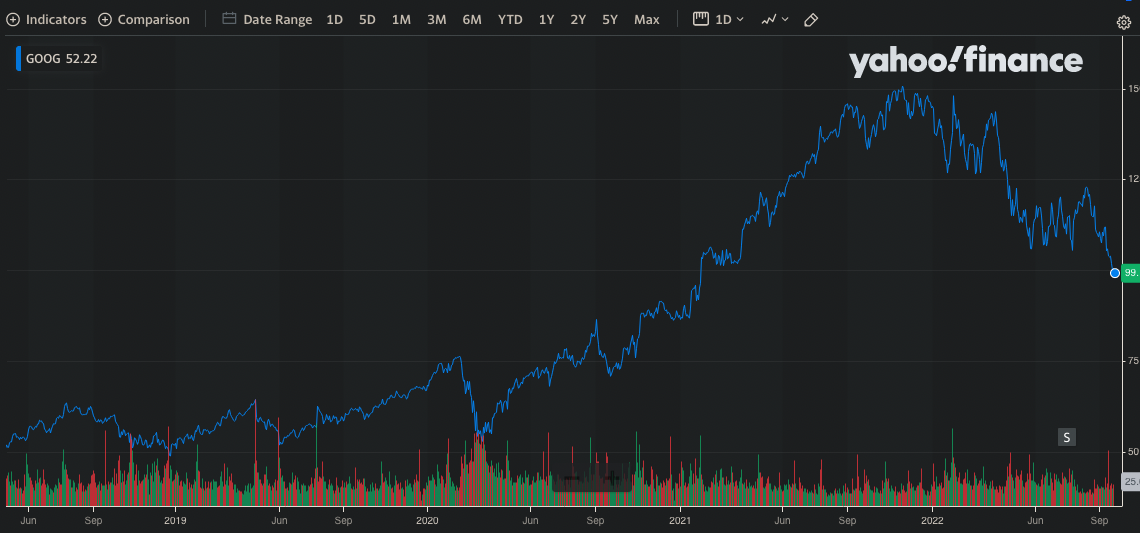
\includegraphics[width = \textwidth]{Images/Finance_Graph.png}
			\end{figure}
		\section{Where and when does the problem initiate and develop, and any other information. (Adding images is preferred)}
			The problem of optimizing buy and sell times for stocks comes from the multitude of external and internal factors involved. For example in business, political, economic, social, and technological changes in the world can all impact stock price negatively or positively. It is impossible for one to describe all changes at once. Rather than attempting to account for each individual affect, a stochastic model models the aggregate of each of these individually minute details.
			\begin{figure}[H]
				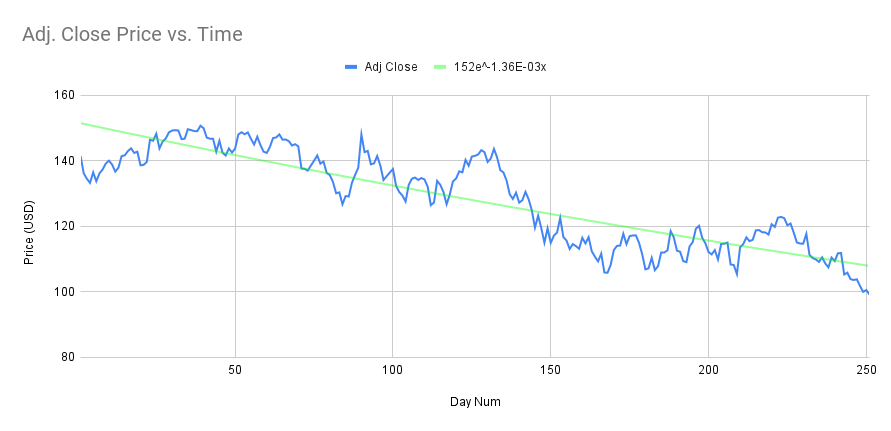
\includegraphics[width = \textwidth]{Images/Sheets_Graph.png}
			\end{figure}
			The graph shows a general downward trend, but on a smaller scale, brief, random fluctuations are clearly visible, attributable to the aforementioned factors. 
		\section{If the problem left without solution what are the side effects?}
			There is no safest way to determine which firm to invest in considering only present market share. Such side effects includes missing qualitative data about the firms that would significantly change stock price. For example, bad public image around a new product release can cause an unforeseen plummet in market-share, which would be unexplained as per the model. 
		\section{Is there any relation between math and the problem? Explain how.}
			In the modern day, the best solutions to optimizing when to buy or sell a stock come from the use of mathematical models. In the Chicago Futures Markets, stochastic models such as that presented here are used to calculate ideal asset prices. The same applied to New York firms, banks also employ math to calculate returns on investments. Many trading services have stochastic indicators built in, meaning that this modeling method used by investors despite them being unaware of it.
		\section{What are the boundary conditions of your model?}
			The price of a stock cannot fall below 0. \\
			For the sake of simplicity, the initial time will be \(t = 0\). It cannot be negative.
		\section{How does Matlab help with differential equations modeling? What are the required Matlab code that need to be programmed to define the model?}
			Matlab makes it far easier to see patterns in the solution of a DE without the need to solve it, which is especially helpful for a DE with nontrivial solutions that are nonelementary. Using loops, it is quite trivial to define a stochastic process in MatLab.
		\section{Input your model using Matlab code then take screenshot of your mathematical model from Matlab to be added to your poster.}
			\begin{figure}[H]
				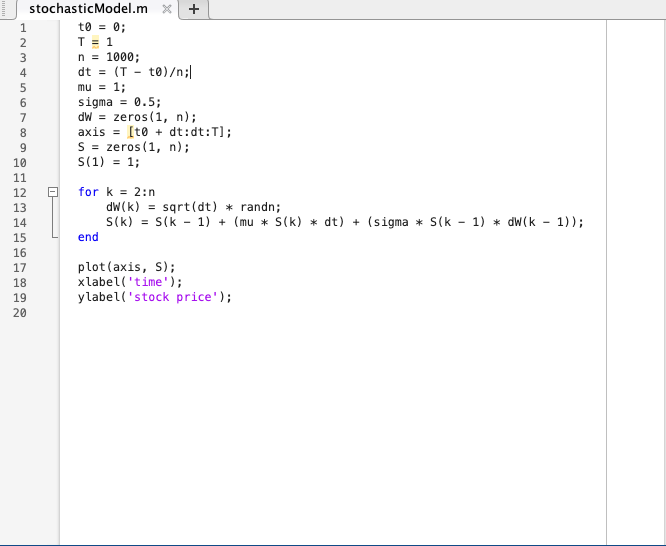
\includegraphics[width = \textwidth]{Images/MatLab_Model.png}
			\end{figure}
			\begin{figure}[H]
				\includegraphics[width = \textwidth]{Images/Matlab_Graph.png}	
			\end{figure}
\end{document}
